\documentclass[]{style/zjuthesis}

\usepackage{color}
\usepackage{fancyvrb}
\newcommand{\VerbBar}{|}
\newcommand{\VERB}{\Verb[commandchars=\\\{\}]}
\DefineVerbatimEnvironment{Highlighting}{Verbatim}{commandchars=\\\{\}}
% Add ',fontsize=\small' for more characters per line
\usepackage{framed}
\definecolor{shadecolor}{RGB}{248,248,248}
\newenvironment{Shaded}{\begin{snugshade}}{\end{snugshade}}
\newcommand{\KeywordTok}[1]{\textcolor[rgb]{0.13,0.29,0.53}{\textbf{{#1}}}}
\newcommand{\DataTypeTok}[1]{\textcolor[rgb]{0.13,0.29,0.53}{{#1}}}
\newcommand{\DecValTok}[1]{\textcolor[rgb]{0.00,0.00,0.81}{{#1}}}
\newcommand{\BaseNTok}[1]{\textcolor[rgb]{0.00,0.00,0.81}{{#1}}}
\newcommand{\FloatTok}[1]{\textcolor[rgb]{0.00,0.00,0.81}{{#1}}}
\newcommand{\ConstantTok}[1]{\textcolor[rgb]{0.00,0.00,0.00}{{#1}}}
\newcommand{\CharTok}[1]{\textcolor[rgb]{0.31,0.60,0.02}{{#1}}}
\newcommand{\SpecialCharTok}[1]{\textcolor[rgb]{0.00,0.00,0.00}{{#1}}}
\newcommand{\StringTok}[1]{\textcolor[rgb]{0.31,0.60,0.02}{{#1}}}
\newcommand{\VerbatimStringTok}[1]{\textcolor[rgb]{0.31,0.60,0.02}{{#1}}}
\newcommand{\SpecialStringTok}[1]{\textcolor[rgb]{0.31,0.60,0.02}{{#1}}}
\newcommand{\ImportTok}[1]{{#1}}
\newcommand{\CommentTok}[1]{\textcolor[rgb]{0.56,0.35,0.01}{\textit{{#1}}}}
\newcommand{\DocumentationTok}[1]{\textcolor[rgb]{0.56,0.35,0.01}{\textbf{\textit{{#1}}}}}
\newcommand{\AnnotationTok}[1]{\textcolor[rgb]{0.56,0.35,0.01}{\textbf{\textit{{#1}}}}}
\newcommand{\CommentVarTok}[1]{\textcolor[rgb]{0.56,0.35,0.01}{\textbf{\textit{{#1}}}}}
\newcommand{\OtherTok}[1]{\textcolor[rgb]{0.56,0.35,0.01}{{#1}}}
\newcommand{\FunctionTok}[1]{\textcolor[rgb]{0.00,0.00,0.00}{{#1}}}
\newcommand{\VariableTok}[1]{\textcolor[rgb]{0.00,0.00,0.00}{{#1}}}
\newcommand{\ControlFlowTok}[1]{\textcolor[rgb]{0.13,0.29,0.53}{\textbf{{#1}}}}
\newcommand{\OperatorTok}[1]{\textcolor[rgb]{0.81,0.36,0.00}{\textbf{{#1}}}}
\newcommand{\BuiltInTok}[1]{{#1}}
\newcommand{\ExtensionTok}[1]{{#1}}
\newcommand{\PreprocessorTok}[1]{\textcolor[rgb]{0.56,0.35,0.01}{\textit{{#1}}}}
\newcommand{\AttributeTok}[1]{\textcolor[rgb]{0.77,0.63,0.00}{{#1}}}
\newcommand{\RegionMarkerTok}[1]{{#1}}
\newcommand{\InformationTok}[1]{\textcolor[rgb]{0.56,0.35,0.01}{\textbf{\textit{{#1}}}}}
\newcommand{\WarningTok}[1]{\textcolor[rgb]{0.56,0.35,0.01}{\textbf{\textit{{#1}}}}}
\newcommand{\AlertTok}[1]{\textcolor[rgb]{0.94,0.16,0.16}{{#1}}}
\newcommand{\ErrorTok}[1]{\textcolor[rgb]{0.64,0.00,0.00}{\textbf{{#1}}}}
\newcommand{\NormalTok}[1]{{#1}}

\usepackage{natbib}
\bibliographystyle{apalike}

% 该文档中首字符为“%”的均为注释行,不会在论文中出现

% 论文默认为双面模式,需单面模式请将第一行换为如下所示:
% \documentclass[oneside]{ZJUthesis}

% 取消目录中链接的颜色,方便打印
% 如需颜色,请将“false”改为“true”
\hypersetup{colorlinks=false}

\begin{document}
%%%%%%%%%%%%%%%%%%%%%%%%%%%%%
%% 正文字体设定
%%%%%%%%%%%%%%%%%%%%%%%%%%%%%
\fangsong

%%%%%%%%%%%%%%%%%%%%%%%%%%%%%
%% 论文封面部分
%%%%%%%%%%%%%%%%%%%%%%%%%%%%%
% 中文封面内容

% 中图分类号
\classification{TM863}

% 单位代码
\serialnumber{10335}

% 密级,如需密级则将其前“%”去掉
\SecretLevel{绝密}

% 学号
\PersonalID{127436}

\title{啊不可挡家}
% 如果标题一行写不下,就写成两行,在下面的命令里写第二行,不需要两行则注释掉
% \titletl{一行写不下写两行}

%英文题目
\Etitle{R bookdownplus}
% 如果一行写不下,同中文题目设定,一行写不下则写两行,不需要就注释掉
% \Etitletl{The Second Line}

% 作者
\author{Peng Zhao}

\degree{壮士}

% 导师
\supervisor{Dr.~Wiki Google}

% 合作导师,如果有的话,去掉注释,
\cpsupervisor{Dr.~Github StackOverflow}

% 专业名称
\major{维修}

% 研究方向
\researchdm{东南西北}

% 所属学院
\institute{雅典学院}

%论文提交日期
\submitdate{664年10月10日}

% 答辨日期
\defenddate{2011年11月1日}

% 生成封面
\makeCoverPage

%%%%%%%%%%%%%%%%%%%%%%%%%%%%%%
%% 中文题名页内容
%%%%%%%%%%%%%%%%%%%%%%%%%%%%%%
% 论文评阅人信息 注意两字名与三字名,两字职称与三字职称的写法,便于对齐
% 多余的名额直接注释掉即可,比如三个评阅人,把评阅人D,E注释掉即可
\reviewersA{丘处机 真人}
\reviewersB{葛 洪 方士}
\reviewersC{寇谦之 天师}
\reviewersD{张三丰 真君}
\reviewersE{孙玄清 真人}

% 答辩委员会信息,如果某一个单位比较长,
% 请在其它较短后面补上{hspace{Xem}},X是比最长的单位名少几个字
% 如果实际人数少于6人,多余的注释掉即可
\chairman{唐三藏  功 佛}
\commissionerA{惠 能  方 丈}
\commissionerB{智 顗  方 丈}
\commissionerC{法 藏  大和尚}
\commissionerD{道 济  和 尚}
\commissionerE{降 龙  尊 者}

% 生成中文题名页
\maketitle


%%%%%%%%%%%%%%%%%%%%%%%%%%%%%%
%% 英文封面内容,硕士论文可不要此页
%%%%%%%%%%%%%%%%%%%%%%%%%%%%%%
% 英文题名
\englishtitle{R bookdownplus}
% 如果题名一行写不下,就写到第二行,不需要则将其注释掉
% \englishtitletl{The Second title Line}

% 评阅人信息,名字,职称,单位尽量用简写,否则会写不下
\EreviewersA{Dr.~A}
\EreviewersB{Dr.~B}
\EreviewersC{Dr.~C}
\EreviewersD{Dr.~D}
\EreviewersE{Dr.~E}

% 答辩委员会信息,同样尽量用简写,否则会写不下
\Echairman{Dr.~O}
\EcommissionerA{Dr.~A}
\EcommissionerB{Dr.~B}
\EcommissionerC{Dr.~C}
\EcommissionerD{Dr.~D}
\EcommissionerE{Dr.~E}

% 生成英文封面
\makeenglishtitle


%%%%%%%%%%%%%%%%%%%%%%%%%%%%%%
%% 原创声明与版权协议页
%%%%%%%%%%%%%%%%%%%%%%%%%%%%%%

% 生成原创声明与版权协议页
\makeOSandCPRTpage


%%%%%%%%%%%%%%%%%%%%%%%%%%%%%%
%% 论文部分开始
%%%%%%%%%%%%%%%%%%%%%%%%%%%%%%
\ZJUfrontmatter



\chapter{勘误表}

诗曰:

\begin{quote}
混沌未分天地乱,茫茫渺渺无人见。 自从盘古破鸿蒙,开辟从兹清浊辨。
覆载群生仰至仁,发明万物皆成善。 欲知造化会元功,须看《西游释厄传》。
\end{quote}

盖闻天地之数,有十二万九千六百岁为一元。将一元分为十二会,乃子、丑、
寅、卯、辰、巳、午、未、申、酉、戌、亥之十二支也。每会该一万八百岁。且就
一日而论:子时得阳气而丑则鸡鸣,寅不通光而卯则日出,辰时食后而巳则挨排,
日午天中而未则西蹉,申时晡而日落酉,戌黄昏而人定亥。譬于大数,若到戌会之
终,则天地昏而万物否矣。再去五千四百岁,交亥会之初,则当黑暗,而两间人
物俱无矣,故曰混沌。又五千四百岁,亥会将终,贞下起元,近子之会,而复逐渐
开明。邵康节曰``冬至子之半,天心无改移。一阳初动处,万物未生时'',到此,天
始有根;再五千四百岁,正当子会,轻清上腾,有日,有月,有星,有辰。日、月、
星、辰,谓之四象,故曰``天开于子''。又经五千四百岁,子会将终,近丑之会,而
逐渐坚实。《易》曰:大哉乾元,至哉坤元!万物资生,乃顺承天。至此,地始凝结。
再五千四百岁,正当丑会,重浊下凝,有水,有火,有山,有石,有土。水、火、
山、石、土,谓之五形,故曰``地辟于丑''。又经五千四百岁,丑会终而寅会之初,
发生万物,历曰``天气下降,地气上升;天地交合,群物皆生''。至此,天清地爽,
阴阳交合。再五千四百岁,正当寅会,生人,生兽,生禽,正谓天地人,三才定位。
故曰``人生于寅''。

\chapter{致谢}

感盘古开辟,三皇治世,五帝定伦,世界之间,遂分为四大部洲:曰东胜神洲、
曰西牛贺洲、曰南赡部洲、曰北俱芦洲。这部书单表东胜神洲。海外有一国土,名
曰傲来国。国近大海,海中有一座名山,唤为花果山。此山乃十洲之祖脉,三岛之
来龙,自开清浊而立,鸿蒙判后而成。真个好山!有词赋为证。赋曰:
势镇汪洋,威宁瑶海:势镇汪洋,潮涌银山鱼入穴;威宁瑶海,波翻雪浪蜃离
渊。水火方隅高积土,东海之处耸崇巅。丹崖怪石,削壁奇峰。丹崖上,彩凤双鸣;
削壁前,麒麟独卧。峰头时听锦鸡鸣,石窟每观龙出入。林中有寿鹿仙狐,树上有
灵禽玄鹤。瑶草奇花不谢,青松翠柏长春。仙桃常结果,修竹每留云。一条涧壑藤
萝密,四面原堤草色新。正是百川会处擎天柱,万劫无移大地根。
那座山正当顶上,有一块仙石。其石有三丈六尺五寸高,有二丈四尺围圆。三丈六
尺五寸高,按周天三百六十五度;二丈四尺围圆,按政历二十四气。上有九窍八孔,
按九宫八卦。四面更无树木遮阴,左右倒有芝兰相衬。盖自开辟以来,每受天真地
秀,日精月华,感之既久,遂有灵通之意。内育仙胞,一日迸裂,产一石卵,似圆
球样大。因见风化作一个石猴。五官俱备,四肢皆全。便就学爬学走,拜了四方。
目运两道金光,射冲斗府。惊动高天上圣大慈仁者玉皇大天尊玄穹高上帝,驾座金
阙云宫灵霄宝殿,聚集仙卿,见有金光焰焰,即命千里眼、顺风耳开南天门观看。
二将果奉旨出门外,看的真,听的明。须臾回报道:``臣奉旨观听金光之处,乃东胜
神洲海东傲来小国之界,有一座花果山,山上有一仙石,石产一卵,见风化一石猴,
在那里拜四方,眼运金光,射冲斗府。如今服饵水食,金光将潜息矣。''玉帝垂赐恩
慈曰:``下方之物,乃天地精华所生,不足为异。''

\chapter{序言}

那猴在山中,却会行走跳跃,食草木,饮涧泉,采山花,觅树果;与狼虫为伴,
虎豹为群,獐鹿为友,猕猿为亲;夜宿石崖之下,朝游峰洞之中。真是``山中无甲
子,寒尽不知年。''

众猴都道:``这股水不知是那里的水。我们今日赶闲无事,顺涧边往上溜头寻看源流,耍子去耶!''喊一声,都拖男挈女,唤弟呼兄,一齐跑来,
顺涧爬山,直至源流之处,乃是一股瀑布飞泉。但见那:

一派白虹起,千寻雪浪飞。

海风吹不断,江月照还依。

冷气分青嶂,余流润翠微。

潺名瀑布,真似挂帘帷。

众猴拍手称扬道:``好水,好水!原来此处远通山脚之下,直接大海之波。''又道:``那
一个有本事的,钻进去寻个源头出来,不伤身体者,我等即拜他为王。''连呼了三声,
忽见丛杂中跳出一个石猴,应声高叫道:``我进去,我进去!''好猴!也是他:

今日芳名显,时来大运通。

有缘居此地,天遣入仙宫。

\chapter{摘要}

你看他瞑目蹲身,将身一纵,径跳入瀑布泉中,忽睁睛抬头观看,那里边却无
水无波,明明朗朗的一架桥梁。他住了身,定了神,仔细再看,原来是座铁板桥。
桥下之水,冲贯于石窍之间,倒挂流出去,遮闭了桥门。却又欠身上桥头,再走再
看,却似有人家住处一般,真个好所在。但见那:

翠藓堆蓝,白云浮玉,光摇片片烟霞。虚窗静室,滑凳板生花。乳窟龙珠倚挂,
萦回满地奇葩。锅灶傍崖存火迹,樽靠案见肴渣。石座石床真可爱,石盆石碗更
堪夸。又见那一竿两竿修竹,三点五点梅花。几树青松常带雨,浑然像个人家。
看罢多时,跳过桥中间,左右观看,只见正当中有一石碣。碣上有一行楷书大字,
镌着``花果山福地,水帘洞洞天''。石猿喜不自胜,急抽身往外便走,复瞑目蹲身,
跳出水外,打了两个呵呵道:``大造化,大造化!''众猴把他围住,问道:``里面怎么
样?水有多深?''石猴道:``没水,没水!原来是一座铁板桥。桥那边是一座天造地
设的家当。''众猴道:``怎见得是个家当?''石猴笑道:``这股水乃是桥下冲贯石窍,
倒挂下来遮闭门户的。桥边有花有树,乃是一座石房。房内有石锅、石灶、石碗、
石盆、石床、石凳。中间一块石碣上,镌着`花果山福地,水帘洞洞天。'真个是我
们安身之处。里面且是宽阔,容得千百口老小。我们都进去住,也省得受老天之气。
这里边:

刮风有处躲,下雨好存身。 霜雪全无惧,雷声永不闻。
烟霞常照耀,祥瑞每蒸熏。 松竹年年秀,奇花日日新。''

\chapter{Abstract}\label{abstract}

众猴听得,个个欢喜。都道:``你还先走,带我们进去,进去!''石猴却又瞑目
蹲身,往里一跳,叫道:``都随我进来!进来!''那些猴有胆大的,都跳进去了;胆小
的,一个个伸头缩颈,抓耳挠腮,大声叫喊,缠一会,也都进去了。跳过桥头,一
个个抢盆夺碗,占灶争床,搬过来,移过去,正是猴性顽劣,再无一个宁时,只搬
得力倦神疲方止。 \ZJUListofFigures

\ZJUListofTables

\chapter{符号}

石猿端坐上面道:``列位呵,`人而无信,不知其可。'你们才说有本事进得来,
出得去,不伤身体者,就拜他为王。我如今进来又出去,出去又进来,寻了这一个
洞天与列位安眠稳睡,各享成家之福,何不拜我为王?''众猴听说,即拱伏无违。
一个个序齿排班,朝上礼拜,都称``千岁大王''。自此,石猿高登王位,将``石''字
儿隐了,遂称美猴王。有诗为证,诗曰:

三阳交泰产群生,仙石胞含日月精。 借卵化猴完大道,假他名姓配丹成。
内观不识因无相,外合明知作有形。 历代人人皆属此,称王称圣任纵横。

\ZJUcontents

\ZJUmainmatter

\chapter{研究背景}

美猴王领一群猿猴、猕猴、马猴等,分派了君臣佐使,朝游花果山,暮宿水帘
洞,合契同情,不入飞鸟之丛,不从走兽之类,独自为王,不胜欢乐。是以\citep{R-base}:

春采百花为饮食,夏寻诸果作生涯。 秋收芋栗延时节,冬觅黄精度岁华。

\begin{Shaded}
\begin{Highlighting}[]
 \KeywordTok{persp}\NormalTok{(x, y, z, }\DataTypeTok{theta =} \DecValTok{120}\NormalTok{, }\DataTypeTok{phi =} \DecValTok{15}\NormalTok{, }\DataTypeTok{scale =} \OtherTok{FALSE}\NormalTok{, }
       \DataTypeTok{axes =} \OtherTok{FALSE}\NormalTok{)}
\end{Highlighting}
\end{Shaded}

\begin{figure}

{\centering 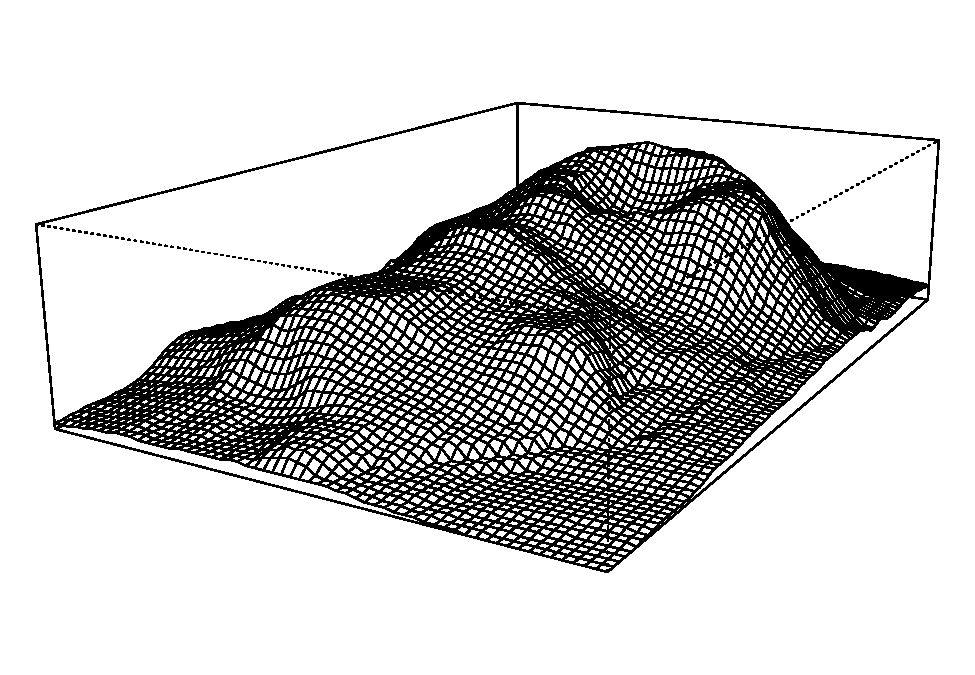
\includegraphics[width=0.6\linewidth]{thesis_zju_zh_files/figure-latex/unnamed-chunk-1-1} 

}

\caption{好图!好图!}\label{fig:unnamed-chunk-1}
\end{figure}

美猴王享乐天真,何期有三五百载。一日,与群猴喜宴之间,忽然忧恼,堕下
泪来。众猴慌忙罗拜道:``大王何为烦恼?''猴王道:``我虽在欢喜之时,却有一点
儿远虑,故此烦恼。''众猴又笑道:``大王好不知足!我等日日欢会,在仙山福地,古
洞神洲,不伏麒麟辖,不伏凤凰管,又不伏人间王位所拘束,自由自在,乃无量之
福,为何远虑而忧也?''猴王道:``今日虽不归人王法律,不惧禽兽威严,将来年老
血衰,暗中有阎王老子管着,一旦身亡,可不枉生世界之中,不得久注天人之内?''
众猴闻此言,一个个掩面悲啼,俱以无常为虑。只见那班部中,忽跳出一个通背猿
猴,厉声高叫道:``大王若是这般远虑,真所谓道心开发也!如今五虫之内,惟有三
等名色,不伏阎王老子所管。''猴王道:``你知那三等人?''猿猴道:``乃是佛与仙与
神圣三者,躲过轮回,不生不灭,与天地山川齐寿。''猴王道:``此三者居于何所?''
猿猴道:``他只在阎浮世界之中,古洞仙山之内。''猴王闻之,满心欢喜,道:``我明
日就辞汝等下山,云游海角,远涉天涯,务必访此三者,学一个不老长生,常躲过
阎君之难。''噫!这句话,顿教跳出轮回网,致使齐天大圣成。众猴鼓掌称扬,都道:
``善哉!善哉!我等明日越岭登山,广寻些果品,大设筵宴送大王也。''\citep{R-bookdown}

\chapter{方法}

次日,众猴果去采仙桃,摘异果,刨山药,精,芝兰香蕙,瑶草奇花,般般
件件,整整齐齐,摆开石凳石桌,排列仙酒仙肴。但见那:

金丸珠弹,红绽黄肥:金丸珠弹腊樱桃,色真甘美;红绽黄肥熟梅子,味果香
酸。鲜龙眼,肉甜皮薄;火荔枝,核小囊红。林檎碧实连枝献,枇杷缃苞带叶擎。
兔头梨子鸡心枣,消渴除烦更解酲。香桃烂杏,美甘甘似玉液琼浆;脆李杨梅,酸
荫荫如脂酥膏酪。红囊黑子熟西瓜,四瓣黄皮大柿子。石榴裂破,丹砂粒现火晶珠;
芋栗剖开,坚硬肉团金玛瑙。胡桃银杏可传茶,椰子葡萄能做酒。榛松榧柰满盘盛,
桔蔗柑橙盈案摆。熟煨山药,烂煮黄精。捣碎茯苓并薏苡,石锅微火漫炊羹。人间
纵有珍羞味,怎比山猴乐更宁?

\begin{table}

\caption{\label{tab:tab1}Here is a nice table!}
\centering
\begin{tabular}[t]{rrrrl}
\toprule
Sepal.Length & Sepal.Width & Petal.Length & Petal.Width & Species\\
\midrule
5.1 & 3.5 & 1.4 & 0.2 & setosa\\
4.9 & 3.0 & 1.4 & 0.2 & setosa\\
4.7 & 3.2 & 1.3 & 0.2 & setosa\\
4.6 & 3.1 & 1.5 & 0.2 & setosa\\
5.0 & 3.6 & 1.4 & 0.2 & setosa\\
\addlinespace
5.4 & 3.9 & 1.7 & 0.4 & setosa\\
4.6 & 3.4 & 1.4 & 0.3 & setosa\\
5.0 & 3.4 & 1.5 & 0.2 & setosa\\
4.4 & 2.9 & 1.4 & 0.2 & setosa\\
4.9 & 3.1 & 1.5 & 0.1 & setosa\\
\addlinespace
5.4 & 3.7 & 1.5 & 0.2 & setosa\\
4.8 & 3.4 & 1.6 & 0.2 & setosa\\
4.8 & 3.0 & 1.4 & 0.1 & setosa\\
4.3 & 3.0 & 1.1 & 0.1 & setosa\\
5.8 & 4.0 & 1.2 & 0.2 & setosa\\
\addlinespace
5.7 & 4.4 & 1.5 & 0.4 & setosa\\
5.4 & 3.9 & 1.3 & 0.4 & setosa\\
5.1 & 3.5 & 1.4 & 0.3 & setosa\\
5.7 & 3.8 & 1.7 & 0.3 & setosa\\
5.1 & 3.8 & 1.5 & 0.3 & setosa\\
\bottomrule
\end{tabular}
\end{table}

群猴尊美猴王上坐,各依齿肩排于下边,一个个轮流上前奉酒奉花,奉果,痛饮了
一日。

次日,美猴王早起,教:``小的们,替我折些枯松,编作筏子,取个竹竿作篙,
收拾些果品之类,我将去也。''果独自登筏,尽力撑开,飘飘荡荡,径向大海波中,
趁天风,来渡南赡部洲地界。这一去,正是那:

天产仙猴道行隆,离山驾筏趁天风。 飘洋过海寻仙道,立志潜心建大功。
有分有缘休俗愿,无忧无虑会元龙。 料应必遇知音者,说破源流万法通。

也是他运至时来,自登木筏之后,连日东南风紧,将他送到西北岸前,乃是南赡部
洲地界。持篙试水,偶得浅水,弃了筏子,跳上岸来,只见海边有人捕鱼、打雁、
挖蛤、淘盐。他走近前,弄个把戏,妆个虎,吓得那些人丢筐弃网,四散奔跑。
将那跑不动的拿住一个,剥了他的衣裳,也学人穿在身上,摇摇摆摆,穿州过府,
在市廛中,学人礼,学人话。朝餐夜宿,一心里访问佛仙神圣之道,觅个长生不老
之方。见世人都是为名为利之徒,更无一个为身命者。正是那:

争名夺利几时休?早起迟眠不自由! 骑着驴骡思骏马,官居宰相望王侯。
只愁衣食耽劳碌,何怕阎君就取勾? 继子荫孙图富贵,更无一个肯回头!

\chapter{结果}

猴王参访仙道,无缘得遇。在于南赡部洲,串长城,游小县,不觉八九年余。
忽行至西洋大海,他想着海外必有神仙。独自个依前作筏,又飘过西海,直至西牛
贺洲地界。登岸遍访多时,忽见一座高山秀丽,林麓幽深。他也不怕狼虫,不惧虎
豹,登山顶上观看。果是好山:
千峰排戟,万仞开屏。日映岚光轻锁翠,雨收黛色冷含青。瘦藤缠老树,古渡
界幽程。奇花瑞草,修竹乔松:修竹乔松,万载常青欺福地;奇花瑞草,四时不谢
赛蓬瀛。幽鸟啼声近,源泉响溜清。重重谷壑芝兰绕,处处崖苔藓生。起伏峦头
龙脉好,必有高人隐姓名。
正观看间,忽闻得林深之处,有人言语,急忙趋步,穿入林中,侧耳而听,原来是
歌唱之声。歌曰:
``观棋柯烂,伐木丁丁,云边谷口徐行。卖薪沽酒,狂笑自陶情。苍径秋高,
对月枕松根,一觉天明。认旧林,登崖过岭,持斧断枯藤。
收来成一担,行歌市上,易米三升。更无些子争竞,时价平平。不会机谋巧算,
没荣辱,恬淡延生。相逢处,非仙即道,静坐讲《黄庭》。''
美猴王听得此言,满心欢喜道:``神仙原来藏在这里!''即忙跳入里面,仔细再看,
乃是一个樵子,在那里举斧砍柴。但看他打扮非常:
头上戴箬笠,乃是新笋初脱之箨;身上穿布衣,乃是木绵拈就之纱;腰间系环
绦,乃是老蚕口吐之丝;足下踏草履,乃是枯莎槎就之爽。手执钢斧,担挽火麻
绳;扳松劈枯树,争似此樵能!

\chapter{讨论}

猴王近前叫道:``老神仙!弟子起手。''那樵汉慌忙丢了斧,转身答礼道:``不当
人,不当人!我拙汉衣食不全,怎敢当`神仙'二字?''猴王道:``你不是神仙,如
何说出神仙的话来?''樵夫道:``我说甚么神仙话?''猴王道:``我才来至林边,只
听的你说:`相逢处非仙即道,静坐讲《黄庭》。'《黄庭》乃道德真言,非神仙而何?''
樵夫笑道:``实不瞒你说,这个词名做《满庭芳》,乃一神仙教我的。那神仙与我舍
下相邻,他见我家事劳苦,日常烦恼,教我遇烦恼时,即把这词儿念念,一则散心,
二则解困。我才有些不足处思虑,故此念念。不期被你听了。''猴王道:``你家既与
神仙相邻,何不从他修行,学得个不老之方,却不是好?''樵夫道:``我一生命苦:
自幼蒙父母养育至八九岁,才知人事,不幸父丧,母亲居孀。再无兄弟姊妹,只我
一人,没奈何,早晚侍奉。如今母老,一发不敢抛离。却又田园荒芜,衣食不足,
只得斫两束柴薪,挑向市廛之间,货几文钱,籴几升米,自炊自造,安排些茶饭,
供养老母,所以不能修行。''猴王道:``据你说起来,乃是一个行孝的君子,向后必
有好处。但望你指与我那神仙住处,却好拜访去也。''樵夫道:``不远,不远。此山
叫做灵台方寸山。山中有座斜月三星洞。那洞中有一个神仙,称名须菩提祖师。那
祖师出去的徒弟,也不计其数,见今还有三四十人从他修行。你顺那条小路儿,向
南行七八里远近,即是他家了。''猴王用手扯住樵夫道:``老兄,你便同我去去。若
还得了好处,决不忘你指引之恩。''樵夫道:``你这汉子,甚不通变。我方才这般与
你说了,你还不省?假若我与你去了,却不误了我的生意,老母何人奉养?我要斫柴,
你自去,自去!''
猴王听说,只得相辞。出深林,找上路径,过一山坡,约有七八里远,果然望
见一座洞府。挺身观看,真好去处,但见:
烟霞散彩,日月摇光。千株老柏,万节修篁:千株老柏带雨,半空青冉冉;万
节修篁含烟,一壑色苍苍。门外奇花布锦,桥边瑶草喷香。石崖突兀青苔润,悬壁
高张翠藓长。时闻仙
鹤唳,每见凤凰翔。仙鹤唳时,声振九霄汉远;凤凰翔起,翎毛五色彩云光。玄
猿白鹿随隐见,金狮玉象任行藏。细观灵福地,真个赛天堂!
又见那洞门紧闭,静悄悄杳无人迹。忽回头,见崖头立一石碑,约有三丈余高,八
尺余阔,上有一行十个大字,乃是``灵台方寸山,斜月三星洞''。美猴王十分欢喜道:
``此间人果是朴实。果有此山此洞。''看勾多时,不敢敲门。且去跳上松枝梢头,摘
松子吃了顽耍。少顷间,只听得呀的一声,洞门开处,里面走出一个仙童,真个丰
姿英伟,像貌清奇,比寻常俗子不同。但见他: 髻双丝绾,宽袍两袖风。
貌和身自别,心与相俱空。 物外长年客,山中永寿童。
一尘全不染,甲子任翻腾。

\chapter{结论}

那童子出得门来,高叫道:``甚么人在此搔扰?''猴王扑的跳下树来,上前躬身道:
``仙童,我是个访道学仙之弟子,更不敢在此搔扰。''仙童笑道:``你是个访道的么?''
猴王道:``是。''童子道:``我家师父,正才下榻,登坛讲道,还未说出原由,就教我
出来开门。说:`外面有个修行的来了,可去接待接待。'想必就是你了?''猴王笑
道:``是我,是我。''童子道:``你跟我进来。''
这猴王整衣端肃,随童子径入洞天深处观看:一层层深阁琼楼,一进进珠宫贝
阙,说不尽那静室幽居,直至瑶台之下。见那菩提祖师端坐在台上,两边有三十个
小仙侍立台下。果然是: 大觉金仙没垢姿,西方妙相祖菩提。
不生不灭三三行,全气全神万万慈。 空寂自然随变化,真如本性任为之。
与天同寿庄严体,历劫明心大法师。
美猴王一见,倒身下拜,磕头不计其数,口中只道:``师父,师父!我弟子志心
朝礼,志心朝礼!''祖师道:``你是那方人氏?且说个乡贯姓名明白,再拜。''猴王道:
``弟子乃东胜神洲傲来国花果山水帘洞人氏。''祖师喝令:``赶出去!他本是个撒诈捣
虚之徒,那里修甚么道果!''猴王慌忙磕头不住道:``弟子是老实之言,决无虚诈。''
祖师道:``你既老实,怎么说东胜神洲?那去处到我这里,隔两重大海,一座南赡部
洲,如何就得到此?''猴王叩头道:``弟子飘洋过海,登界游方,有十数个年头,方
才访到此处。''祖师道:``既是逐渐行来的也罢。你姓甚么?''猴王又道:``我无性。
人若骂我,我也不恼;若打我,我也不嗔,只是陪个礼儿就罢了。一生无性。''祖师
道:``不是这个性。你父母原来姓甚么?''猴王道:``我也无父母。''祖师道:``既无
父母,想是树上生的?''猴王道:``我虽不是树上生,却是石里长的。我只记得花果
山上有一块仙石,其年石破,我便生也。''祖师闻言暗喜,道:``这等说,却是个天
地生成的。你起来走走我看。''猴王纵身跳起,拐呀拐的走了两遍。祖师笑道:``你
身躯虽是鄙陋,却像个食松果的猢狲。我与你就身上取个姓氏,意思教你姓`猢'。
猢字去了个兽傍,乃是个古月。古者,老也;月者,阴也。老阴不能化育,教你姓
`狲'倒好。狲字去了兽傍,乃是个子系。子者,儿男也;系者,婴细也。正合婴
儿之本论。教你姓`孙'罢。''猴王听说,满心欢喜,朝上叩头道:``好,好,好!今
日方知姓也。万望师父慈悲!既然有姓,再乞赐个名字,却好呼唤。''祖师道:``我门
中有十二个字,分派起名,到你乃第十辈之小徒矣。''猴王道:``那十二个字?''祖
师道:``乃`广大智慧,真如性海,颖悟圆觉'十二字。排到你,正当`悟'字。与
你起个法名叫做`孙悟空',好么?''猴王笑道:``好,好,好!自今就叫做孙悟空也!''
正是: 鸿蒙初辟原无姓,打破顽空须悟空。
毕竟不知向后修些甚么道果,且听下回分解。 \# 参考文献

\appendix \addcontentsline{toc}{chapter}{\appendixname}


\chapter{原始数据}\label{data}


\bibliography{bib/bib}


\end{document}
